\clearpage
\section{Probability Distribution}
\begin{colbox}
    \begin{enumerate}
        \item Create and diplay a gaussian distribution of 10,000 measurements of 0 volt with a single voltmeter and a standard deviation of 0.01.
        \item Show a histogram of 50 measurements for a measurement of 0 volt which is performed with 50 different measurement devices.
        \item Show a combined measurement of 0 volt performed as follows: 20 measurements with a device whose standard deviation is 0.1, 10 with a device with a deviation of 0.05, 5 with an std to 0.01, and 15 with an std of 0.02.
        \item We'll use the measurement device from part 1 and measure the following set of voltages, each voltage measured 5 times: 0.5v, 1.0v, 3.9v, 7.8v, 10v, 13.4v, 15.2v, 17.5v, 21.1v, 25v. Show the results as a scatter plot (the wanted voltage as a function of the measured voltage).
        \item Performed a linear fit for the measurements in part 4 and use the tools you know to estimate how good the fit is.
    \end{enumerate}
\end{colbox}
\subsection{0 volts}
\begin{figure}[!htb]
    \centering
    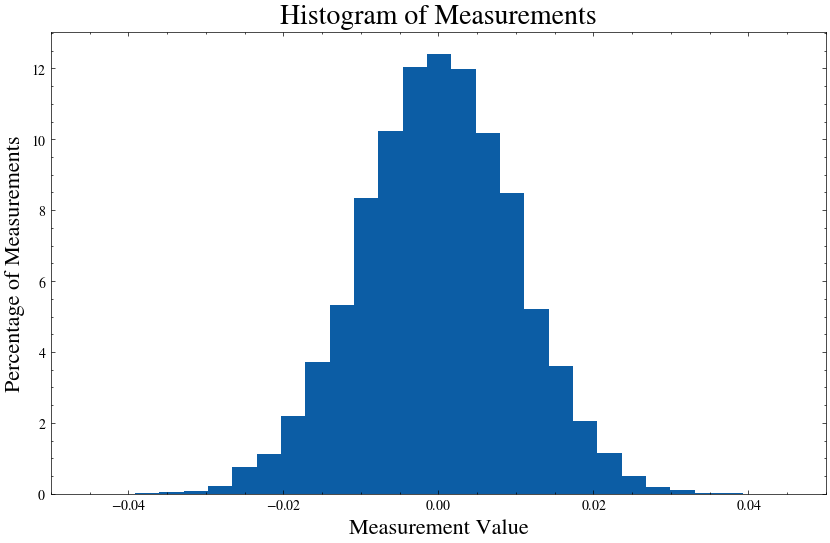
\includegraphics[width=0.9\textwidth]{q2p1.png}
    \caption{Histogram of \(10,000\) measurements from a gaussian distribution with \(\mu=0\) and \(\sigma=0.01\).}
\end{figure}
\newpage
\subsection{50 measurements}
\begin{figure}[!htb]
    \centering
    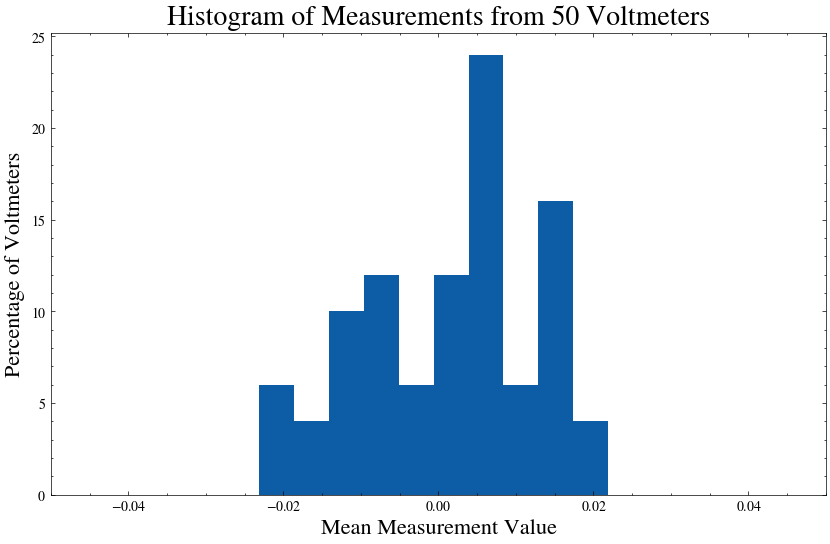
\includegraphics[width=0.9\textwidth]{q2p2.png}
    \caption{Histogram of \(50\) measurements using 50 different gaussian distributions with \(\mu=0\) and \(\sigma=0.01\).}
\end{figure}
\subsection{composite measurement}
\begin{figure}[!htb]
    \centering
    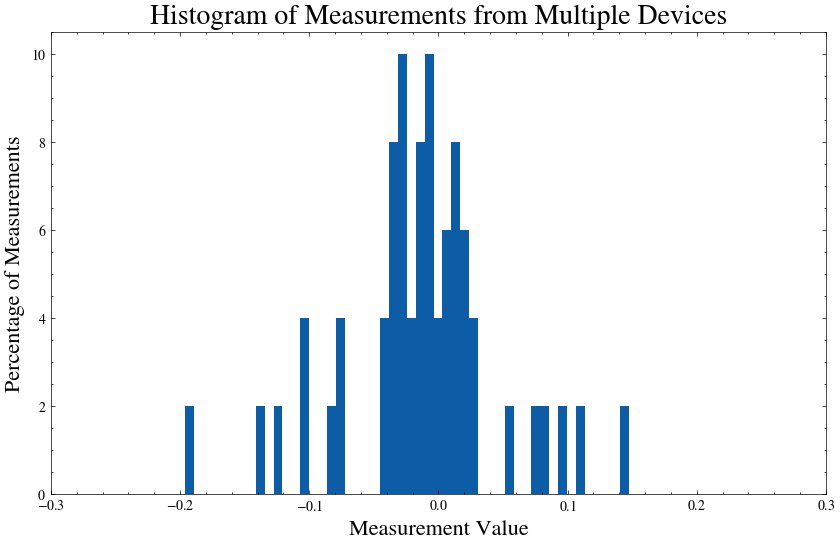
\includegraphics[width=0.85\textwidth]{q2p3.png}
    \caption{Histogram of measurements of \(0V\), where 20 have \(\sigma=0.1\), 10 have \(\sigma=0.05\), 5 have \(\sigma=0.01\), and 15 have \(\sigma=0.02\).}
\end{figure}
Using the calculations for the weighted mean and uncertainty on it we find
\begin{align}
    \overline{x} = 0.004854 && \sigma_{\overline{x}} = 0.003270
\end{align}
\subsection{Multiple Voltages}
\begin{figure}[!htb]
    \centering
    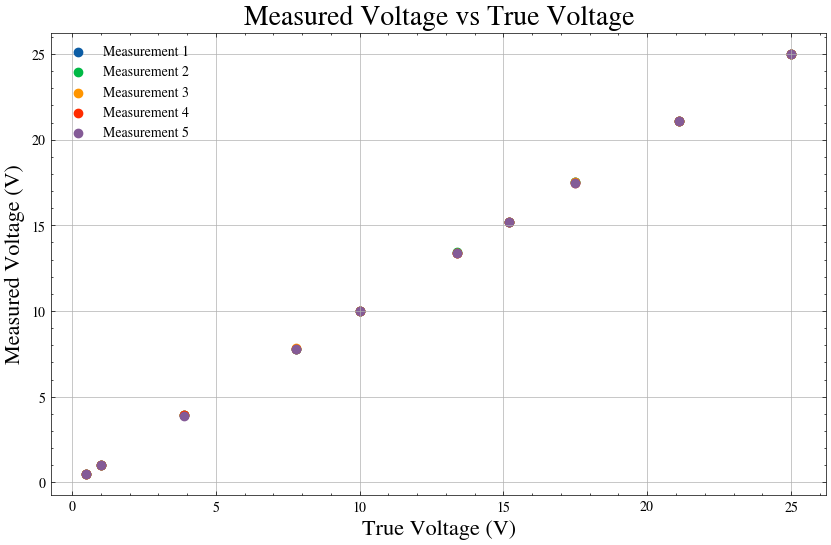
\includegraphics[width=0.85\textwidth]{q2p4.png}
    \caption{Histogram of measurements of several voltages, each measured 5 times, all with the same device.}
\end{figure}
\subsection{Linear Fit}
Peforming a linear fit we find
\begin{align}
    y = \ins{0.9999\pm0.0002}x + \ins{0.0019\pm0.0002} && R^2=0.999
\end{align}